\chapter{Analysis Overview}\label{ch:analysis_overview}

\section{The RPV UDD signature}\label{sec:signal_of_interest}

This analysis is a search for pair-produced gluinos decaying to a large number of standard model quarks via R-parity-violating decays, as described in~\ref{subsec:rpv_gluino}.
In the direct decay model, each gluino decays directly to three standard-model quarks via an effective vertex with an off-shell squark propagator.
In the cascade decay model, each gluino first decays to a neutralino and two quarks, and the neutralino then decays similarly to three quarks vai the RPV effective vertex.
Both types of signal events would result in a large number of high-$p_{T}$ jets in the detector, because they have a large number of quarks in the final state, and each quark must be boosted due to the large mass of the gluinos.
Figure~\ref{fig:analysis_rpv_decays} shows the diagrams for the two signal models under consideration.

\begin{figure}[ht!]
    \centering
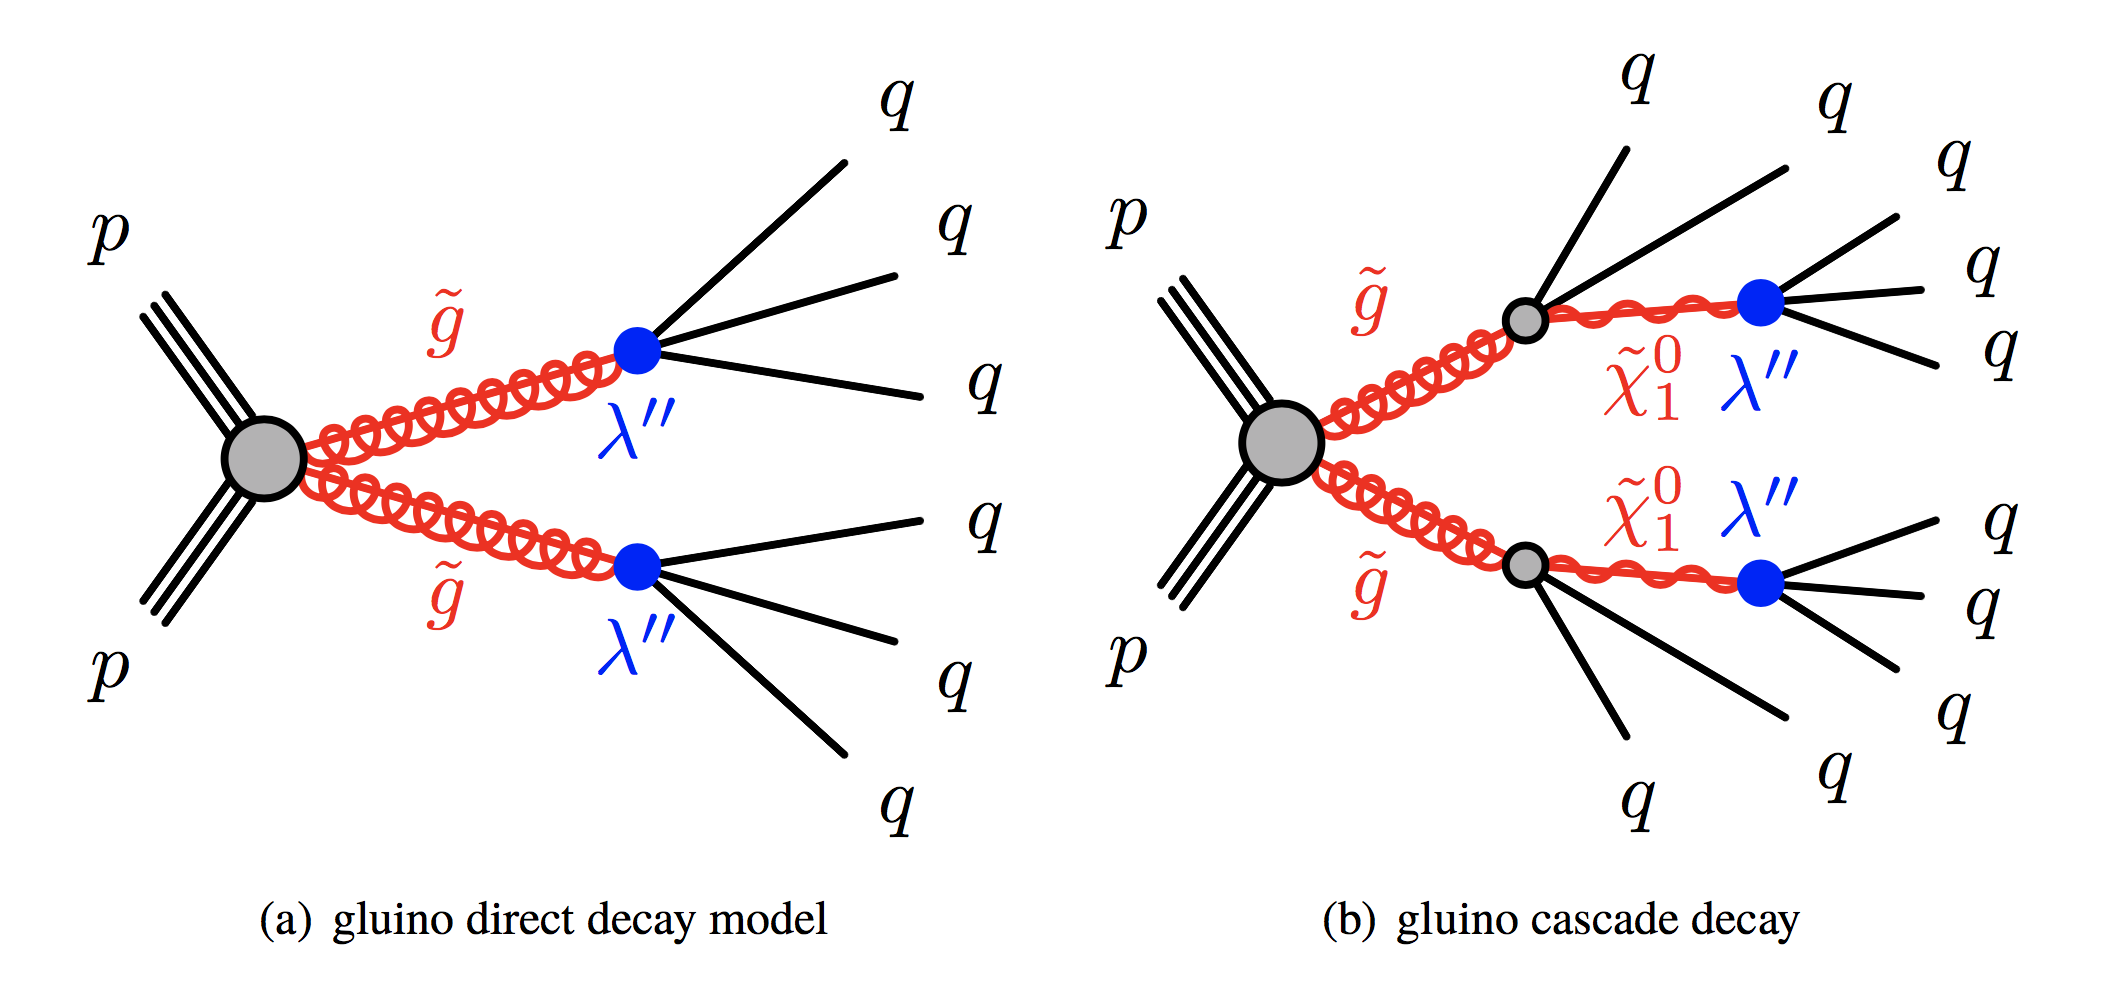
\includegraphics[width=0.95\linewidth]{decay_diagrams_combined}
\caption{Diagrams for the two decay processes that are the subject of this search. The direct decay (left) and cascade decay (right)
both involve effective RPV vertices containing off-shell squark propagators.}
\label{fig:analysis_rpv_decays}
\end{figure}

\section{Previous searches and limits}\label{sec:run1_limits}

A similar search was performed using $20.3~fb^{-1}$ of $8~TeV$ ATLAS data from Run 1, and limits were set on the gluino and neutralino masses~\cite{run1-multijet}.
Two different strategies were employed in this analysis.
The first strategy looked for an excess of events with high small-$R$ jet multiplicities.
Signal regions required $\geq6$ or $\geq7$ jets, and different $b$-jet multiplicity requirements were applied to create signal regions sensitive to different heavy-flavor branching fractions.
In the jet-counting analysis, backgrounds were estimated by extrapolating event yields from lower jet multiplicity regions, using a scaling factor derived from multijet Monte Carlo.
This strategy was mainly aimed at the direct-decay model.

The second strategy used the sum of large-$R$ jet masses as discriminating variable, and was mainly aimed at the cascade-decay model.
This strategy derived jet mass templates from signal-depleted control regions, and used those templates to generate the estimated background mass distribution in the signal regions.

For the cascade decay model, the observed limit on the gluino mass ranged from $800~GeV$ to $1~TeV$, depending on the neutralino mass.
Figure~\ref{fig:run1_cascade_limits} shows the $95\%$ CL lower bounds in the $(m_{\tilde{g}}, m_{\tilde{\chi}})$ plane from the search for the cascade-decay signal.
For the direct decay model, different limits were placed on the gluino mass for different assumptions about the flavor composition of the final states.
In the case of light-quark only decays, gluino masses above $917~GeV$ were excluded~\cite{run1-multijet}.
Figure~\ref{fig:run1_direct_limits} shows the $95\%$ CL upper bounds on the cross-section for the direct decay model over a range of gluino masses, for various assumptions about the flavor composition of the final states.

\begin{figure}[!ht]\centering
    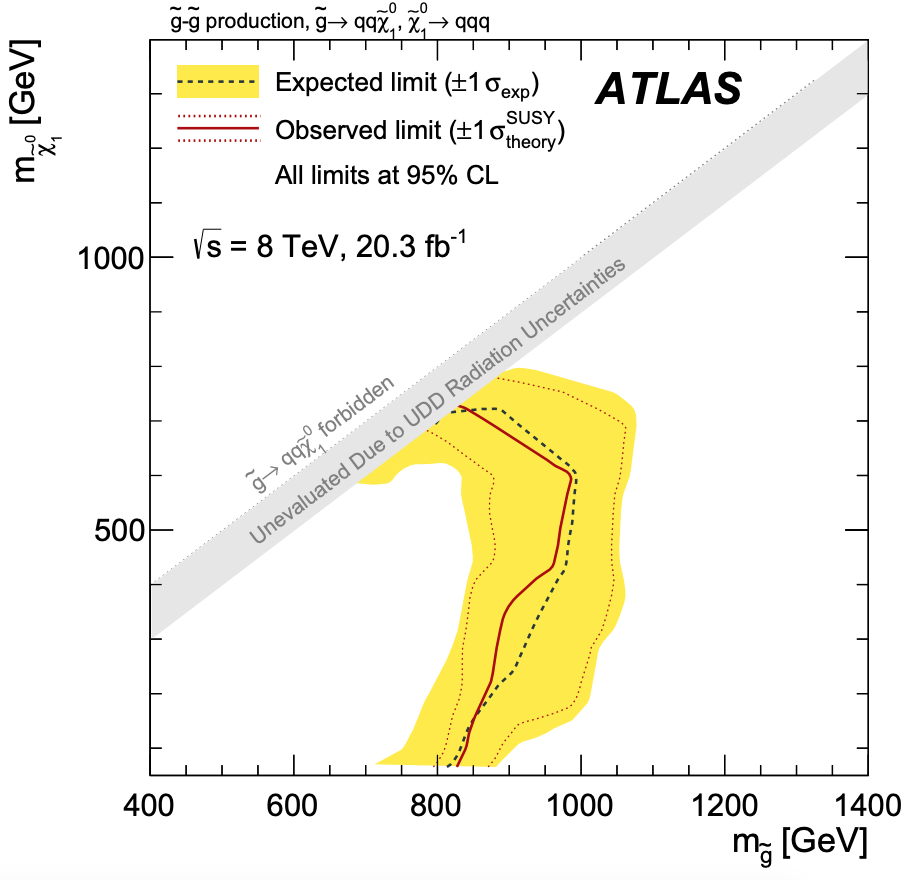
\includegraphics[width=0.6\textwidth]{analysis_run1_cascade_limits}
    \caption{Observed and expected limits in the $(m_{\tilde{g}}, m_{\tilde{\chi}})$ plane for the cascade-decay model in ATLAS Run 1 with $\sqrt{s}=8~TeV$~\cite{run1-multijet}.
    }
    \label{fig:run1_cascade_limits}
\end{figure}

\begin{figure}[!ht]\centering
    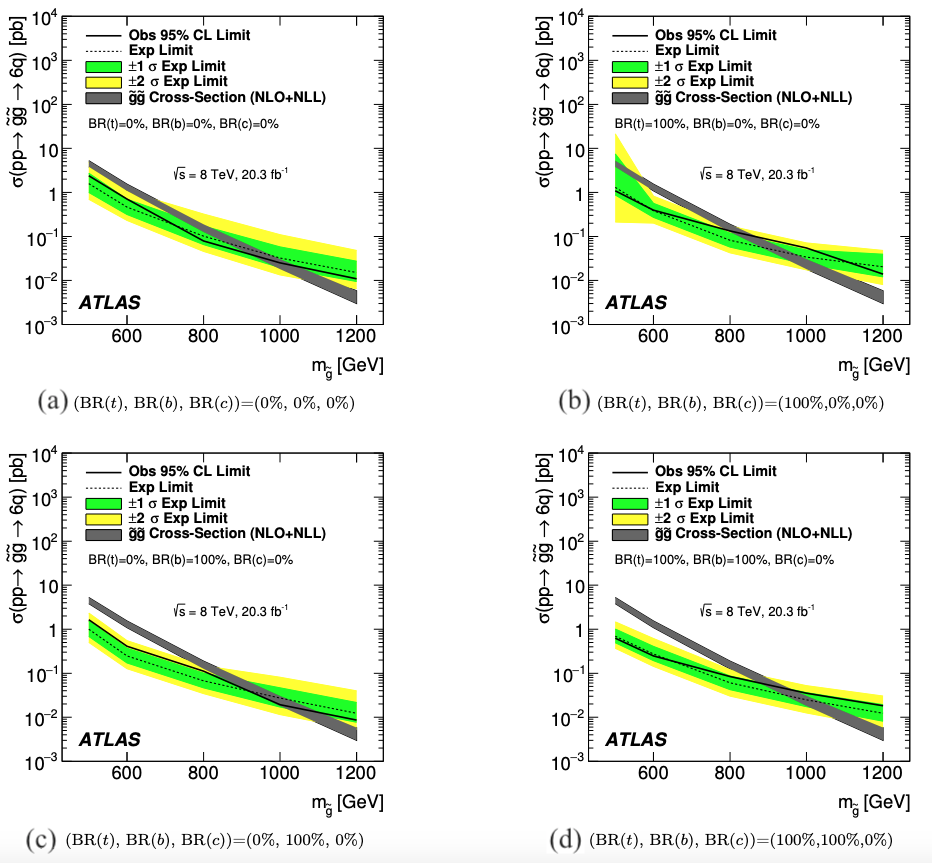
\includegraphics[width=0.9\textwidth]{analysis_run1_direct_limits}
    \caption{Observed and expected limits on $m_{\tilde{g}})$, along with theoretical cross-section for the direct-decay model in ATLAS Run 1 with $\sqrt{s}=8~TeV$~\cite{run1-multijet}.
    Different limits are set for four different branching fraction scenarios.
    In sub-figure (a), only light-quark decays are allowed.
    In sub-figure (b), each gluino decay results in a top quark in the final state.
    In sub-figure (c), each gluino decay results in a bottom quark in the final state.
    In sub-figure (d), each gluino decay results in both a top and a bottom quark in the final state~\cite{run1-multijet}.}
    \label{fig:run1_direct_limits}
\end{figure}

In Run 1, CMS also performed a search for RPV decays of gluinos with high jet-multiplicity final states~\cite{analysis-cms-run1}.
The analysis assumed that $\lambda''_{tbs}$ is the largest of the UDD coupling constants, motivated by minimal flavor-violating (MFV) SUSY~\cite{susy-mfv}.
Based on this assumption, the analysis specifically looked at the direct-decay model, in which the gluinos each decay to exactly one top, one bottom, and one strange quark, via an off-shell stop.
The analysis looked at events with zero or one-lepton final states high jet multiplicity, using $b$-jet multiplicity as a discriminating variable\cite{analysis-cms-run1}.
For the fully-hadronic channel, the dominant background was QCD multijets, and for the single-lepton channel, the dominant background was from $t\bar{t}$.
In both cases, backgrounds were estimated from Monte Carlo with corrections derived from control-region data.
The single-lepton channel ended up setting the strongest limit on the gluino mass, excluding $pp\rightarrow\tilde{g}\tilde{g}\rightarrow tbs$ for gluinos with mass less than $1.03~TeV$~\cite{analysis-cms-run1}.

The increased luminosity and center-of-mass energy of collisions in Run 2 creates an opportunity to extend the reach of the search for RPV SUSY in multijet final states.
Figure~\ref{fig:results_ten_quark_limits} shows the expected limit for gluino masses under the cascade decay scenario increasing to up to $1.9~TeV$, and up to $1.2~TeV$ under the direct-decay scenario.

\section{Search strategy and discriminating variables}\label{sec:search_strategy}

The search strategy is similar to the total-jet-mass analysis from ATLAS Run 1~\cite{run1-multijet}.
Signal regions include events with a large number of high-mass large-$R$ jets, and backgrounds are estimated using jet mass templates derived from control region data.
The primary discriminating variable is $M_{J}^{\Sigma}$, defined as:

\begin{equation}
    M_{J}^{\Sigma} = \sum_{j=1}^{4}m_{jet}^j
\end{equation}
where $m_{jet}$ is large-$R$ jet mass, and the sum is over the first four highest-$p_{T}$ jets in the event.
Large-$R$ jets are reconstructed with $R=1.0$ and are required to have $p_{T}>200~GeV$ and $|\eta|<2.0$.
In the case where an event has fewer than 4 large-$R$ jets passing the kinematic thresholds, the sum over all large-$R$ jets in the event is used.
This observable is sensitive to the signal because there are large numbers of quarks in the final state, and each quark is likely to have high $p_{T}$ due to the large gluino mass.
Background events, which mainly come from QCD multijet production, tend to have much lower jet mass on average, as explained in~\ref{sec:jet_mass}.
Unlike with the boosted scenarios described in~\ref{sec:jet_mass}, the jet mass for signal events does not come from capturing the decay products of a single boosted heavy object in an individual jet.
Instead, the high jet mass in signal events results from the high probability that two or more decay products, possibly from different parent particles, can accidentally overlap inside the same large-$R$ jet.
$M_{J}^{\Sigma}$ provides good separation between signal and background because it takes into account both the energy and angular structure of an event, unlike a purely energy-dependent observable like $H_{T}$~\cite{hook-mj,elhedri-mj}.

The second discriminating variable is $|\Delta \eta_{12}|$, the pseudorapidity difference between the first two leading jets in an event.
For events with high jet multiplicity, the signal has smaller $|\Delta \eta_{12}|$ than the background.

Distributions of the two discriminating variables are shown in figure~\ref{fig:MJ_dEta_distributions} for data as well as background and signal Monte Carlo.
The different event generators all show similar $M_{J}^{\Sigma}$ distributions for QCD multijets, and a clear difference can be seen between the signal and background distributions.
For signal events, the location of the $M_{J}^{\Sigma}$ peak depends on the gluino mass, moving to higher values for larger masses.
The shape of the $|\Delta \eta_{12}|$ distribution does not depend as strongly on the gluino mass, but there is still a clear difference between the signal and background distributions.
In the analysis, a requirement of small $|\Delta \eta_{12}|<1.4$ can therefore be used to further suppress the background.

\begin{figure}[!ht]
    \centering
    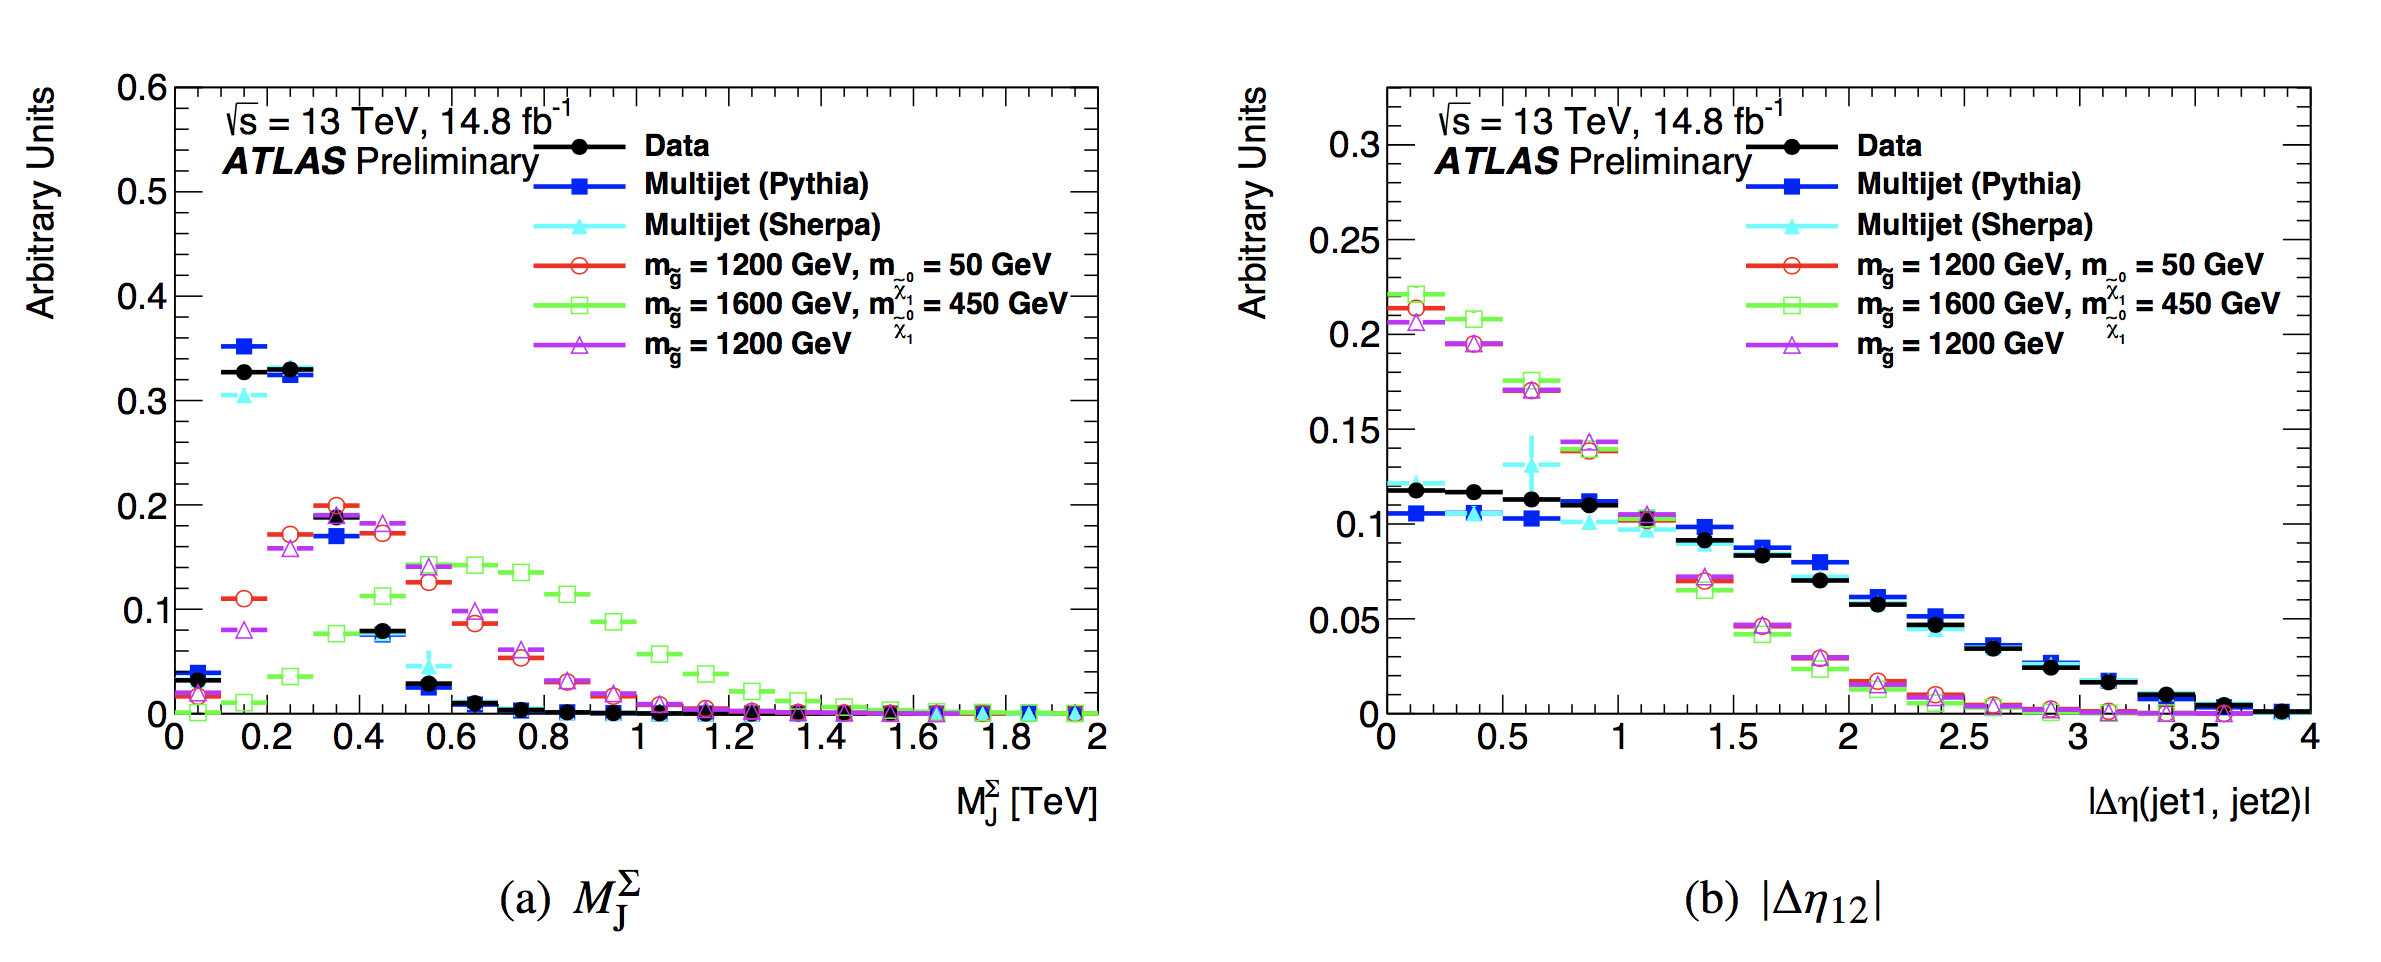
\includegraphics[width=0.9\textwidth]{MJ_dEta_distributions_combined}
    \caption{Distributions of the two main discriminating observables, (a) the scalar sum of the four leading large-R jets, $M_{J}^{\Sigma}$ and (b) the difference in pseudorapidity between the two leading jets, $|\Delta\eta_{12}|$.
    Selected events have $\geq 4$ large-R jets.
    Distributions are shown for both data and simulated signal and background samples.
    The red and green signal distributions are for the cascade decay mode, and the violet distribution is the direct decay mode, for the superpartner masses indicated~\cite{paper-plb}.}
    \label{fig:MJ_dEta_distributions}
\end{figure}

A data-driven method is used to predict the background yield in the signal regions, as well as the uncertainties on those predictions.
The method assumes that for background events, the probably distribution for the mass of an individual jet depends mainly on the $p_{T}$, $\eta$, and flavor of that jet, and does not depend strongly on other details of the event kinematics.
Using this assumption, templates for jet mass can be built from jet in a background-dominated region and used to predict the mass distribution for jets in signal regions.
Templates are binned in $p_{T}$ and $\eta$, and are derived separately for $b$-matched and non-$b$-matched jets.
Each template is a histogram of jet mass within a certain range of $p_{T}$ and $\eta$.
The histogram is used as the probability distribution for a jet to have a certain mass, conditional on its $p_{T}$, $\eta$, and flavor.

Randomized jet masses, known as dressed masses, are generated from these templates for each jet in the kinematic sample.
Summing the dressed masses for each of the up to four leading jets in an event gives the dressed $M_{J}^{\Sigma}$ for that event.
The dressed $M_{J}^{\Sigma}$ distribution for each signal region is used to estimate the expected background contribution to that region.

The method is similar to that used in the Run-1 version of the analysis~\cite{run1-multijet}, with a few important differences.
In the Run-1 analysis, the templates were smoothed with a kernel density estimate before sampling the dressed masses.
In this version of the analysis, the templates remain binned.
This allows for an estimate of the statistical uncertainty from the control sample size.
By Poisson fluctuating each template bin before sampling, the statistical uncertainty is propagated to the dressed $M_J^{\Sigma}$ distributions.
Secondly, in the Run-1 version of the analysis, two separate sets of templates were generated: one set for the leading two jets in each event, and a separate set for the third leading jet.
In this analysis, the templates are instead divided into b-matched and non-b-matched jets.
The discrepancy in template shape between b-matched and non-b-matched jets was seen to be larger than that between the third leading jet and first two leading jets.
Finally, the Run-1 version of the analysis used Monte-Carlo non-closure as one contribution to the background systematic uncertainty.
In this analysis, a data-driven method is used instead.
This is due to the fact that the sample size of available simulated data was not large enough to make an accurate estimate of the non-closure.
More details of the template-based background estimation method and how uncertainties are derived from data will be given in~\ref{sec:jet_mass_templates}.